  %2017-09-27
  \subsection{Сложное движение твердого тела}
  Рассмотрим неподвижную систему отсчета $OXYZ$, подвижную $O_1xyz$, и систему, связанную с телом $S\xi\eta\zeta$.
  \begin{df} Абсолютная угловая скорость - угловая скорость $S\xi\eta\zeta$ относительно $OXYZ$\end{df}
  \begin{df} Относительная угловая скорость - угловая скорость $S\xi\eta\zeta$ относительно $O_1xyz$\end{df}
  \begin{df} Переносная угловая скорость - угловая скорость $Oxyz$ относительно $OXYZ$\end{df}  
  \begin{teo}[О сложении угловых скоростей] $\v{\omega}_{\text{абс}} = \v{\omega}_{\text{отн}} + \v{\omega}_{\text{пер}}$ \end{teo}
  \begin{proof}
  $$ \v{v}_A^{\text{абс}} = \v{v}_A^{\text{отн}} + \v{v}_A^{\text{пер}} $$
  $$ \v{v}_B^{\text{абс}} = \v{v}_B^{\text{отн}} + \v{v}_B^{\text{пер}} $$
  $$ \v{v}_B^{\text{абс}} = \v{v}_A^\text{абс} + [\v{\omega}_{\text{абс}}, \overline{AB}] $$

  $$ \v{v}_B^{\text{отн}} = \v{v}_A^\text{отн} + [\v{\omega}_{\text{отн}}, \overline{AB}] $$

  $$ \v{v}_B^{\text{пер}} = \v{v}_A^\text{пер} + [\v{\omega}_{\text{пер}}, \overline{AB}] $$
  $$ \Rightarrow 0 = 0 + [\v{\omega}_{\text{абс}} - \v{\omega}_{\text{отн}} - \v{\omega}_{\text{пер}}, \overline{AB}] = 0,~~ \forall \overline{AB} \Leftrightarrow \v{\omega}_{\text{абс}} = \v{\omega}_{\text{отн}} + \v{\omega}_{\text{пер}} $$
  \end{proof}

  \begin{ntc}
  $\frac{d\v{\omega}_{\text{пер}}}{dt} = \dot{\v{\omega}}_\text{пер} + [\v{\omega}_\text{пер}, \v{\omega}_\text{пер}] = \dot{\v{\omega}}_\text{пер} $
  \end{ntc}

  \begin{teo}[О сложении угловых ускорений] 
  $\v{\varepsilon}_{\text{абс}} = \v{\varepsilon}_{\text{отн}} + \v{\varepsilon}_{\text{пер}} + [\v{\omega}_{\text{пер}}, \v{\omega}_\text{отн}]$, где $\v{\varepsilon}_{\text{абс}} = \frac{d}{dt}\v{\omega}_{\text{абс}}$, $\v{\varepsilon}_{\text{отн}} = \dot{\v{\omega}}_{\text{отн}}$, $\v{\varepsilon}_{\text{пер}} = \frac{d}{dt}\v{\omega}_{\text{пер}} = \dot{\v{\omega}}_{\text{пер}}$
  \end{teo}

  \begin{proof}
  $$ \v{\varepsilon}_{\text{абс}} = \frac{d}{dt}(\v{\omega}_{\text{отн}} + \v{\omega}_{\text{пер}}) = $$ 
  $$ = \dot{\v{\omega}}_{\text{отн}} + [\v{\omega}_{\text{пер}}, \v{\omega}_{\text{отн}}] + \frac{d}{dt}\v{\omega}_{\text{пер}} =
  \v{\varepsilon}_{\text{отн}} + [\v{\omega}_{\text{пер}}, \v{\omega}_{\text{отн}}] + \v{\varepsilon}_{\text{пер}} $$ 

  \end{proof}

  \subsubsection{Несколько подвижных систем отсчета}~
  
  \noindent $OXYZ$ - неподвижная СО \\
  $Ox_1y_1z_1$, $Ox_2y_2z_2$ , $\ldots Ox_ny_nz_n$ - подвижные СО \\
  $S\xi\eta\zeta$ - связана с телом \\
  $\v{\omega}$ - угловая скорость $S\xi\eta\zeta$ относительно $OXYZ$ \\
  Тогда: $\v{\omega} = \sum\limits_{i = 1}^{n} \v{\omega_i}$
  
  \subsection{Кинематические формулы Эйлера}
  \begin{figure}[H]
  \centering
  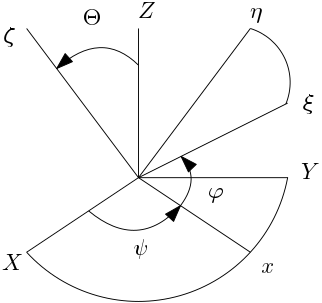
\includegraphics[width=5cm]{fig13.png} 
  \end{figure}  

  \begin{df} $ Ox = (OXY)\cap(O\xi\eta) $ - линия узлов \end{df}
  \begin{df} $\psi = \angle(Ox, OX)$ - угол прецессии \end{df}
  \begin{df} $\Theta = \angle (O\zeta, OZ)$ - угол нутации \end{df}
  \begin{df} $\varphi = \angle (Ox, O\xi)$ - угол собственного вращения \end{df}
  \begin{df} $\{\psi, \Theta, \varphi\}$ - углы Эйлера \end{df}

  Повороты:
  $ OXYZ \xrightarrow{\psi, OZ} OxyZ \xrightarrow{\Theta, Ox} Oxy\zeta \xrightarrow{\varphi, O\zeta} O\xi\eta\zeta $

  $\v{\omega} = \dot{\psi}\v{e}_Z + \dot{\Theta}\v{e}_x + \dot{\varphi}\v{e}_{\zeta}$

  $\v{e}_x = \cos \varphi \v{e}_{\xi} - \sin \varphi \v{e}_{\eta}$
  
  $\v{e}_z = \cos \Theta \v{e}_{\zeta} + \sin \Theta ( \sin \varphi \v{e}_{\xi} + \cos \varphi \v{e}_{\eta} )$
  $$\begin{array}{rcl}\v{\omega} & = & \dot\psi(\sin \Theta \sin \varphi \v{e}_{\xi} + \sin \Theta \cos \varphi \v{e}_{\eta} + \cos \Theta \v{e}_{\zeta}) \\
  & + & \dot \Theta (\cos \varphi \v{e}_{\xi} - \sin \varphi\v{e}_{\eta}) \\
  & + & \dot{\varphi}\v{e}_{\zeta} = \omega_{\xi}\v{e}_{\xi} + \omega_{\eta}\v{e}_{\eta} + \omega_{\zeta}\v{e}_{\zeta} \\
  \end{array}$$

  $$
  \begin{cases}
  \v{\omega}_{\xi} = \dot{\psi}\sin\Theta \sin\varphi + \dot{\Theta}\cos\varphi \\
  \v{\omega}_{\eta} = \dot{\psi}\sin\Theta \cos\varphi - \dot{\Theta}\sin\varphi \\
  \v{\omega}_{\zeta} = \dot{\psi}\cos\Theta + \dot{\varphi} \\
  \end{cases}
  \text{ - кинематические формулы Эйлера}
  $$

  \begin{df} 
  Движение твердого тела называется прецессией, если некоторая ось, неподвижная в теле, в абсолютном пространстве движется по поверхности неподвижного кругового конуса. $\dot{\Theta} = 0$. Если $\dot {\psi} = const$, $\dot {\varphi} = const$, то прецессия называется регулярной.
  \end{df}

  \section{Алгебра кватернионов}
  \begin{df} Алгеброй над полем называется векторное пространство над этим полем, снабженное билинейной операцией умножения. \end{df}
  \begin{xmp} ~

  $\underline{n=2}$(\textit{Комплексные числа}). $z_1 = a + bi$, $z_2 = c + di$ 

  $$ z_1z_2 = (ac - bd) + (ad + bc)i $$

  \end{xmp}
  $\underline{n=4}$(\textit{Алгебра кватернионов})

  \begin{flalign*}
  & \Lambda = \lambda_0 \v{i}_0 + \lambda_1 \v{i}_1 + \lambda_2 \v{i}_2 + \lambda_3 \v{i}_3 \in \mathbb{H} &\\
  & \{\v{i}_0, \v{i}_1, \v{i}_2, \v{i}_3\} \text{ - базис} &\\ 
  & \Lambda = \lambda_0 + \overline{\lambda} &\\
  & i_0 \circ i_k = i_k \quad k = \overline{1, 3},~ i_0 \circ i_0 = 1 &\\
  & i_k \circ i_m = -(i_k, i_m) + [i_k, i_m] \quad k, m \in \{1,2,3\}, \qquad  \text{В частности, $i_k \circ i_k = -1$}&\\
  & \overline{\lambda} \circ \overline{\mu} = (\lambda_1 \v{i}_1 + \lambda_2 \v{i}_2 + \lambda_3 \v{i}_3) \circ (\mu_1 \v{i}_1 + \mu_2 \v{i}_2 + \mu_3 \v{i}_3) = -(\overline{\lambda}, \overline{\mu}) + [\overline{\lambda}, \overline{\mu}] &\\
  & \Lambda \circ M = (\lambda + \overline{\lambda}) \circ (\mu + \overline{\mu}) = \lambda_0 \mu_0 + \lambda_0\overline{\mu} + \overline{\lambda}\mu_0 - (\overline{\lambda}, \overline{\mu}) + [\overline{\lambda}, \overline{\mu}] &\\
  \end{flalign*}
  \paragraph{Свойства:}
  \begin{enumerate}
    \item $(\Lambda \circ M) \circ N = \Lambda \circ (M \circ N)$
    \item $(\Lambda + M) \circ N = \Lambda \circ N + M \circ N $
    \item $\Lambda \circ M \neq M \circ \Lambda$
  \end{enumerate}

